% AUTORIGHTS
% Copyright (C) 2007 Princeton University
%       
% This file is part of Ferret Toolkit.
% 
% Ferret Toolkit is free software; you can redistribute it and/or modify
% it under the terms of the GNU General Public License as published by
% the Free Software Foundation; either version 2, or (at your option)
% any later version.
% 
% This program is distributed in the hope that it will be useful,
% but WITHOUT ANY WARRANTY; without even the implied warranty of
% MERCHANTABILITY or FITNESS FOR A PARTICULAR PURPOSE.  See the
% GNU General Public License for more details.
% 
% You should have received a copy of the GNU General Public License
% along with this program; if not, write to the Free Software Foundation,
% Inc., 51 Franklin Street, Fifth Floor, Boston, MA 02110-1301, USA.
\section {Toolkit Overview}

Figure \ref{fig:arch} shows the general architecture of the CASS toolkit.
For the first release, we are going to release a library (consists of
indexing modules, cass\_table modules, distance\_function modules
 and storage layer) as well
as a reference implementation which can be used to do content-aware
similarity search.

\begin{figure}[ht!]
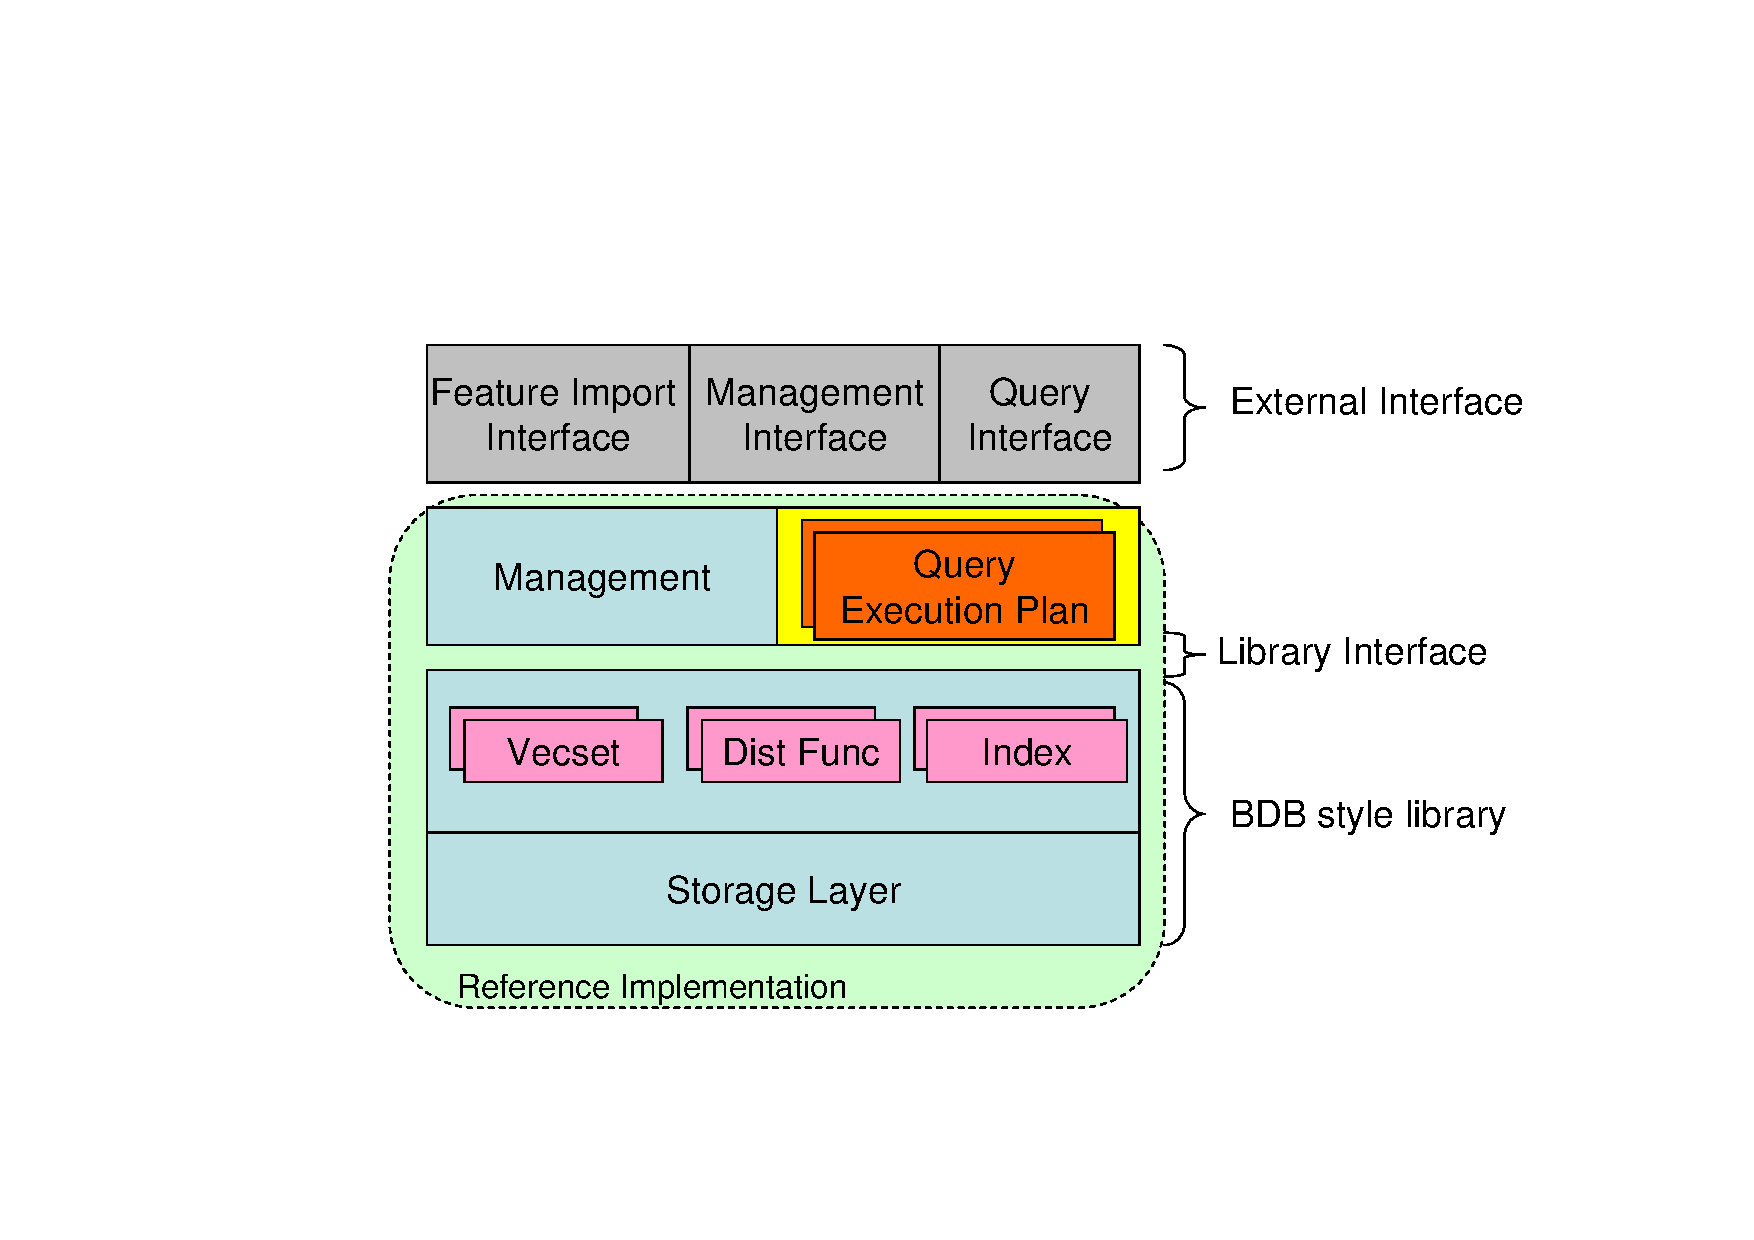
\includegraphics[clip=true,trim=1in 0.6in 0.1in 1.7in, width=0.8\textwidth]{cass_arch}
\caption{CASS Toolkit architecture}
\label{fig:arch}
\end{figure}

The following modules are part of the reference system for the
content-aware similarity search.
\begin{itemize}
\item Storage layer: Provides persistent storage for the system. It
  will support consistency via explicit checkpointing from
  application level. 
\item CASS\_table: They are DB table-like containers which store
  collection of cass\_vecsets which are feature representation of data\_objs.
\item Index: They are DB index like containers which store the index
  for cass\_table. Of note, they could index on cass\_vecset or
  cass\_vec.
\item Management: This is internal management module to manage
  index, cass\_tables, their associations and their placement
  (in-memory or not, where on disk)
\item Query Execution Plan: They are different ways of answering the
  query using different method to combine indexes and
  cass\_tables.
\end{itemize}

The following modules are external interfaces to the CASS system:
\begin{itemize}
\item Feature import interface: To import feature data into the system. 
\item Management interface: To manage and customize the CASS system.
\item Query interface: To satisfy end users' similarity search query.
\end{itemize}



